\section{Methodology} \label{method}
\noindent A method for determining the level of non-determinism of an engine is presented in this section and the working flow of the method is shown in Figure \ref{method_diagram}. Each of the steps in the method is elaborated in the following subsections.
\begin{figure*}[h!]
    \centering
    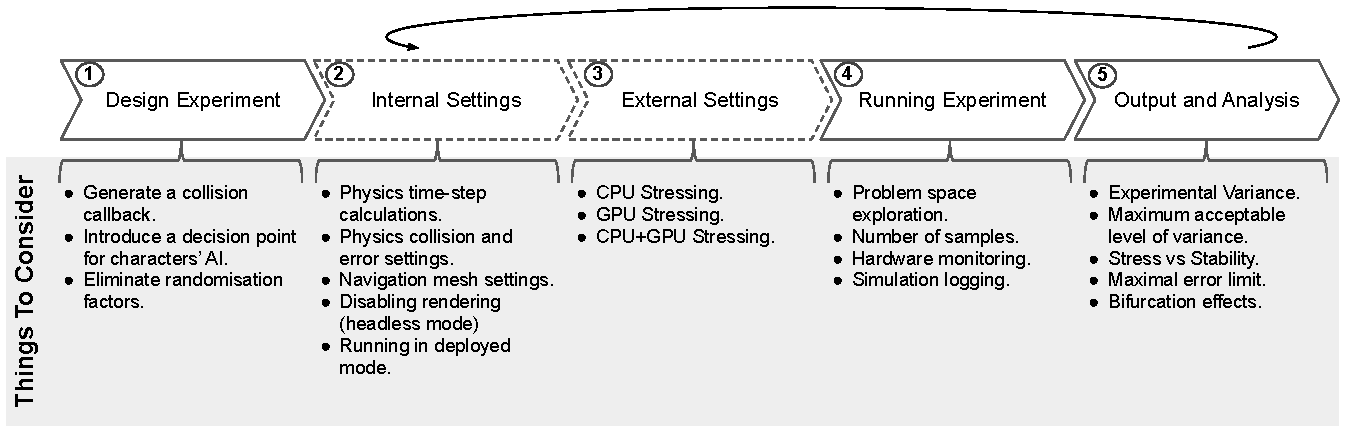
\includegraphics[width=0.99\linewidth]{Other/Figures/MethodologyDiagramCropped.pdf}
    \caption{Shows a flow diagram of the methodology proposed to define the level of non-determinism of a physics engine.}

    \label{method_diagram}
\end{figure*}
\subsection{Design experiment}
\noindent When designing the experiment(s) one needs to bare in mind the following two questions: i) Is the engine deterministic? ii) If not, how does its level of non-determinism vary?\\\\
In simulation, actors can either follow a series of trajectory way points or they get given the destination and their AI path plans to that destination. 
Thus, given that an engine is non-deterministic one needs to set up an experiment that would stress the engine in order to determine how its level of non-determinism vary. This is best done by generating collision callbacks, because that is when engines' do a lot of calculations to determine the response after the collision. Another approach, if AI is used for path planning instead of just following predefined trajectory way points, is to introduce a decision point for the AI.\\\\
It is crucial to also make sure that any randomisation factors are eliminated in the experiment.

\subsection{Internal settings}
\noindent There are several error and physics collision internal settings in physics engines that can be tweaked to enhance the level of non-determinism. \\\\
\noindent Increasing the physics time-step calculations, which is increasing the number of calculations per unit time, would improve the level of non-determinism since the physics sequence will be more finely defined; but on the other hand this would be more computationally expensive. However, in such applications of V\&V of CAV simulations, the computational cost should be of less concern compared to the importance of repeatability of tests. \\\\
\noindent If the experiment setup includes the usage of the physics engine's AI then altering the navigation mesh settings in the engine, like increasing the granularity of the mesh or changing the mesh type; can improve the level of non-determinism as a result of allowing the AI to navigate in a more well defined space.  \\\\
\noindent Disabling rendering or running in headless mode is a way of attempting to decouple the rendering engine from the physics engine, which theoretically should affect positively the repeatablility of tests. 
The downside of most physics engines is that they do not provide a headless mode in the editor setup, thus this could make running in headless mode a real challenge for verification engineers.  \\\\
\noindent Running in editor or deployed mode can sometimes cause massive differences in performance, with deployed mode being worse, mostly due to the way settings get packaged when in deployed mode.

\subsection{External settings}
\noindent Running other programs in the background, like having a web browser open, or running the physics engine in the background while performing other tasks on the same machine does also have an effect; because it alters the CPU and GPU utilisation of tasks.\\\\ 
\noindent Trying to run stress experiments on computers by running other programs makes it difficult to control experiments since the utilisation would be inconsistent, nonetheless, there exists dedicated stress utilisation programs which provide consistent CPU and GPU stressing. Note, however, that during running these tests computers should be left alone not be used for any other purposes apart from running the experiments.

\subsection{Running experiment}
\noindent When it comes to running the experiment itself, things that one should consider  are the problem space exploration; the number of runs that should be executed to get reliable results; the frequency of logging data of actors; and possibly having a program to monitor the hardware utilisation.
% Problem exploration, there is too many variables that one can play with. do statistical analysis some.... some of them get problematic...

\subsection{Output and analysis}
\noindent Once the experiments are run, the logged data is post processed to find the variance in the logged data between the different runs. Note that bifurcation effects can cause a jump in the variance, so it is worth plotting the different logged paths in order to determine if there are any bifurcation effects.\\\\
This whole process is repeated for various internal and external settings. 
Then various plots can be created to identify and engine's level of non-determinsim. 
Thereon, it would be up to the verification engineers to determine where they want to define the line below which the level of non-determinism would be acceptable, and thus know at which levels of computational utilisation they can guarantee to run repeatable experiments.   

